\chapter{Introducción}
\label{cap:Introduccion}

\section{Motivación}
\label{sec:Motivacion}
En los últimos años, la Ingeniería del Software ha observado notables cambios a la hora de desarrollar proyectos software. Tradicionalmente, el modelo de desarrollo de software utilizado consistía en la coordinación de diferentes equipos de trabajo en un mismo edificio (\emph{Desarrollo Colocalizado}); posteriormente, estos equipos de trabajo pasaron a organizarse entre diferentes edificios de una o varias ciudades, pero siempre centralizados en un mismo país (\emph{Desarrollo Distribuido}). Sin embargo, en la actualidad y debido a la globalización, cada vez más compañías separadas geográficamente colaboran para desarrollar software hasta traspasar fronteras llegando a un nivel mundial, por lo que se ha evolucionado hacia un modelo de desarrollo mucho más globalizado y deslocalizado, conocido como \emph{Desarrollo Global de Software} (DGS), o en inglés \emph{Global Software Development} (GSD) \cite{piattini2014desarrollo}.

El DGS está teniendo cada vez más aceptación entre los profesionales. Esta tendencia consiste en la colaboración entre diferentes equipos de desarrollo (Fig.~\ref{fig:DGSFiguraMapa}), los cuales se encuentran ubicados alrededor del mundo en diferentes ciudades, países y continentes. Estos grupos de trabajo pueden pertenecer a distintas organizaciones, pero trabajan conjuntamente en un mismo proyecto software. En el proyecto podrá existir tanto una comunicación \emph{asíncrona} como \emph{síncrona} entre los equipos de trabajo, lo cual dependerá de una serie de características del proyecto \cite{prikladnicki2008improving}. 

\begin{figure}[htb]
	\centering
	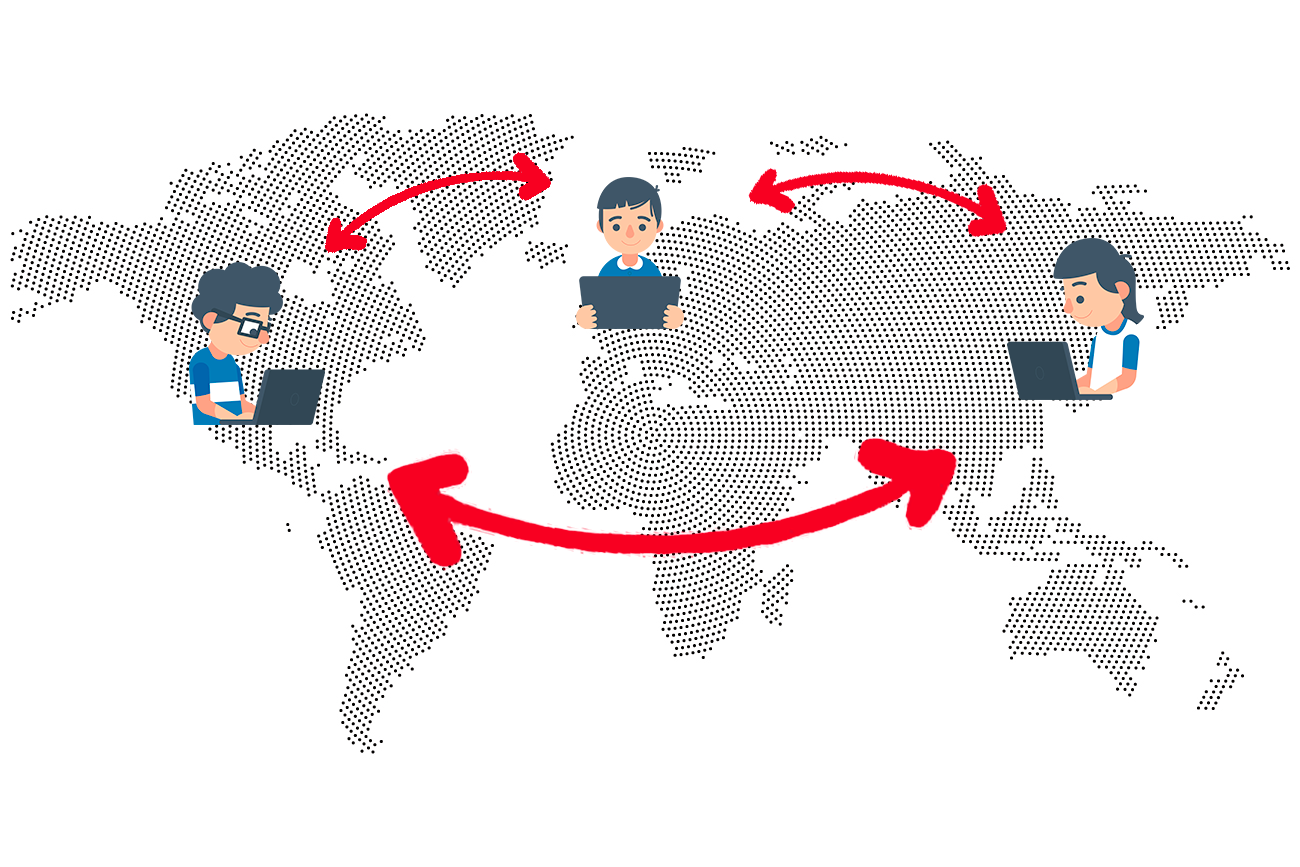
\includegraphics[width=0.75\linewidth]{DGSFiguraMapa}
	\caption[Colaboración mundial en el DGS]{En el DGS diferentes equipos de desarrollo colaboran a nivel mundial en un mismo proyecto}
	\label{fig:DGSFiguraMapa}
\end{figure} 

Gradualmente, esta tendencia esta cogiendo cada vez más fuerza en el campo de la ingeniería del software, considerándose una norma en el desarrollo de software \cite{bosnic2019assessing}. Esto es debido a que las organizaciones pueden conseguir grandes beneficios utilizando este nuevo modelo de desarrollo, ya que la principal ganancia que se consigue con su uso es la reducción en el coste económico de los proyectos, debido a que se suelen buscar territorios donde la mano de obra cualificada es barata y fácilmente disponible \cite{monasor2010preparing}. Además, se pueden encontrar otros beneficios notables como pueden ser el acercamiento del desarrollo del software al cliente y al mercado local, la reducción del período necesario para el desarrollo del software al maximizar la productividad y la expansión hacia la inclusión de trabajadores mayormente cualificados en sus actividades de desarrollo \cite{aagerfalk2008benefits}.

Sin embargo, acompañando a las anteriores ventajas que se pueden conseguir con los proyectos DGS, existen una serie de inconvenientes, los cuales son causados, principalmente, a las diferencias existentes en este tipo de proyectos las cuales podemos dividir en cuatro clases: las \emph{diferencias lingüísticas}, la \emph{distancia geográfica}, la \emph{diferencia cultural} y la coexistencia de diferentes \emph{zonas horarias}; haciendo mucho más difícil el consenso y entendimiento común \cite{monasor2010preparing}. Estas diferencias acentúan la problemática de administrar y gestionar un proyecto software, apareciendo así los tres principales desafíos en la gestión de proyectos DGS (Fig.~\ref{fig:desafiosDGS}), también llamado en \cite{piattini2014desarrollo} como las tres ces:
\begin{itemize}
	\item Desafíos en la comunicación. Los equipos de trabajo deben mantener una comunicación adecuada y activa, con el fin de llevar a cabo un intercambio constante de información y conocimientos. 
	\item Desafíos en la coordinación. Las tareas deben estar sincronizadas, para no sufrir retrasos y alcanzar objetivos e intereses comunes. 
	\item Desafíos en el control. El proyecto debe ser gestionado constantemente y confirmar que se cumplen fechas de entrega, estándares, presupuestos, etc.; además de solventar posibles contratiempos que puedan ocurrir durante el ciclo de vida del proyecto. 
\end{itemize}

\begin{figure}[htb]
	\centering
	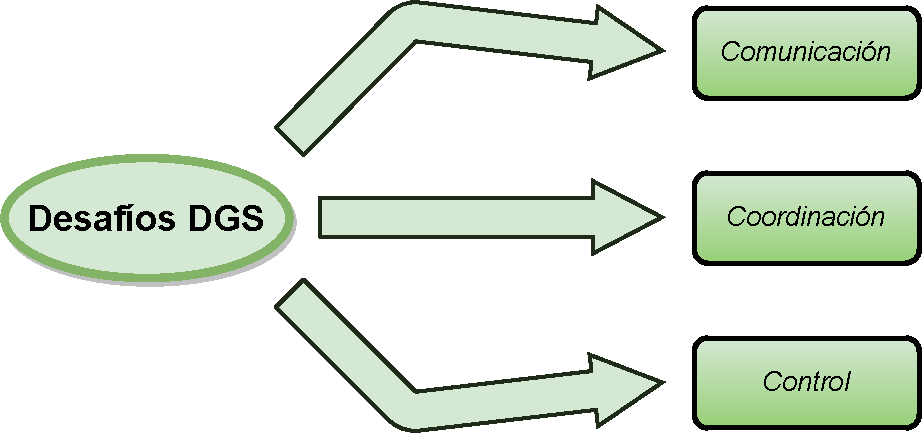
\includegraphics[width=0.75\linewidth]{desafiosDGS}
	\caption[Desafíos en los proyectos DGS]{Los tres principales desafíos en la gestión de proyectos DGS}
	\label{fig:desafiosDGS}
\end{figure}

Estos inconvenientes y desafíos complican la gestión de este tipo de proyectos, lo que puede implicar en el retraso de tareas o incluso en la cancelación del mismo, ya que según la literatura, muchos proyectos DGS terminan fracasando. Según \cite{lino2015project}, la principal causa del fracaso de estos proyectos es debido a la imperfecta y dificultosa gestión de los mismos. Es por esto, que para conseguir los beneficios que nos ofrece el DGS es necesario que los jefes de proyecto posean grandes conocimientos y experiencia en la gestión de este tipo de proyectos, además de contar con una serie de habilidades (no solo técnicas), para hacer frente a los posibles contratiempos que puedan ocurrir en el ciclo de vida del proyecto y conseguir la finalización exitosa del mismo.

\newpage
\section{Propuesta}
\label{sec:Propuesta}

Existe una gran problemática con esta nueva tendencia de desarrollar software y un elevado número de proyectos terminan fracasando, y son escasos aquellos que consiguen finalizar exitosamente. Esta situación se debe a que la educación en Ingeniería del Software no suele tener en cuenta las capacidades necesarias para afrontar los desafíos que conllevan los proyectos DGS, lo que implica que futuros ingenieros del software no posean dichas capacidades \cite{monasor2010preparing}. Por otro lado, cabe destacar que este modelo de desarrollo está siendo cada vez más utilizado en la práctica y es posible que, en un futuro, se termine convirtiendo en un estándar, por lo que es necesario entrenar a nuestros estudiantes para afrontar estas dificultades, ya que se terminarán convirtiendo en los futuros ingenieros de DGS \cite{beecham2017best}.

La gestión y administración es el pilar principal sobre el que gira un proyecto, y en especial un proyecto DGS, ya que es necesaria la organización de un gran número de trabajadores y equipos de desarrollo, a los que se le añade la problemática de gestionar diferentes factores a tener en cuenta como la separación geográfica, la cultura de los diferentes países involucrados en el proyecto o el horario de trabajo en cada país, es por esto que gestionar este tipo de proyectos eficientemente, es un autentico reto. Por lo tanto, es evidente la necesidad de que existan jefes de proyecto altamente cualificados en la gestión de proyectos DGS, para que puedan afrontar la administración del mismo con éxito, solventando todos los impedimentos que puedan ocasionarse. Sin embargo, en la actualidad es complicado encontrar a jefes de proyectos que posean una gran experiencia en proyectos DGS y por lo tanto posean todas las habilidades necesarias. Como consecuencia, son muchas las organizaciones que se han quejado de la carencia de habilidades y experiencia en los jefes de proyecto DGS, y por lo tanto, la consideran la principal  causa del elevado fracaso de estos proyectos \cite{lino2015project}.

Por consiguiente, es necesario educar y enseñar a nuestro futuros ingenieros de software conocimientos sobre DGS en general, y que conozcan la forma correcta de gestionar este tipo de proyectos mediante el entrenamiento de ciertas habilidades. En contraposición, llevar a cabo el entrenamiento y enseñanza de estas habilidades y conocimientos no es una tarea sencilla, puesto que se precisaría la necesidad de introducir a ingenieros de software inexpertos en proyectos reales (para que adquieran esa experiencia necesaria) y por consiguiente las compañías no estén dispuestas a invertir sus recursos en este tipo de programas de entrenamiento. Esta posición de las compañías es debido a que se pueden poner en riesgo proyectos en curso, además de resultar complejo reproducir un escenario real en un entorno de educación \cite{monasor2010preparing}.

En cualquier caso, hay diferentes formas de llevar a cabo la educación de diferentes conocimientos prácticos y el entrenamiento de ciertas habilidades, sin que esto pueda afectar, en nuestro caso, a un proyecto real. En el campo de la \emph{Educación en la Ingeniería de Software} se han realizado avances, buscando la manera más efectiva de educar ciertos conocimientos a estudiantes de ingeniería de software, apareciendo métodos tradicionales como proyectos finales, combinación de diferentes técnicas de enseñanza como aprendizaje basado en proyectos \cite{alabbadi2016proposed}, innovadoras estrategias como las clases volteadas \cite{choi2013applying}, o darle un enfoque relacionado con el uso de juegos, apareciendo el termino de \emph{Gamificación} \cite{connolly2007application}.

Dentro de la gamificación podemos encontrar diferentes tendencias como pueden ser: los cursos académicos \cite{murphy2008distance}, los entornos de aprendizaje \cite{burnell2002teaching} o las aplicaciones que presentan escenarios reales, conocidos como \emph{Juegos Serios} (JSs) \cite{meneely2009preparing}. En especial, los JSs (también llamados juegos educativos), según \cite{calderon2018multivocal}, "consisten en juegos que van más allá del puro entretenimiento y constituyen una potente herramienta que permite a sus jugadores experimentar y aprender de sus errores, adquiriendo así experiencia y conocimientos". Los JSs sirven de ayuda en el proceso de aprendizaje, en donde se simulan entornos virtuales, sin el riesgo de estar en un entorno real \cite{lino2015project, beecham2017best, calderon2018multivocal}.

En consecuencia, este \emph{Trabajo Fin de Carrera} (TFG) se centrará en el desarrollo de un JS, llamado \emph{GLOBAL-MANAGER}. El objetivo de GLOBAL-MANAGER será el de ayudar a estudiante en ingeniería de software a adquirir y entrenar ciertas habilidades (en especial aquellas no técnicas también llamadas \emph{soft skills}) necesarias cuando se aborda el papel de jefe de proyecto DGS. El jugador tendrá que abordar la gestión de un proyecto DGS ficticio desde el comienzo hasta la entrega del producto software al cliente, tratando de resolver los diferentes impedimentos que se puedan ocasionar en el ciclo de vida. De esta manera, los jugadores podrán adquirir experiencia de una manera sencilla, barata e independiente, permitiéndoles afrontar con éxito un futuro trabajo en la gestión de un proyecto DGS. En la figura \ref{fig:funcionamientoJuego}, se muestra un diagrama del funcionamiento que se permite conseguir con el desarrollo de la propuesta anteriormente citada.

\begin{figure}[htb]
	\centering
	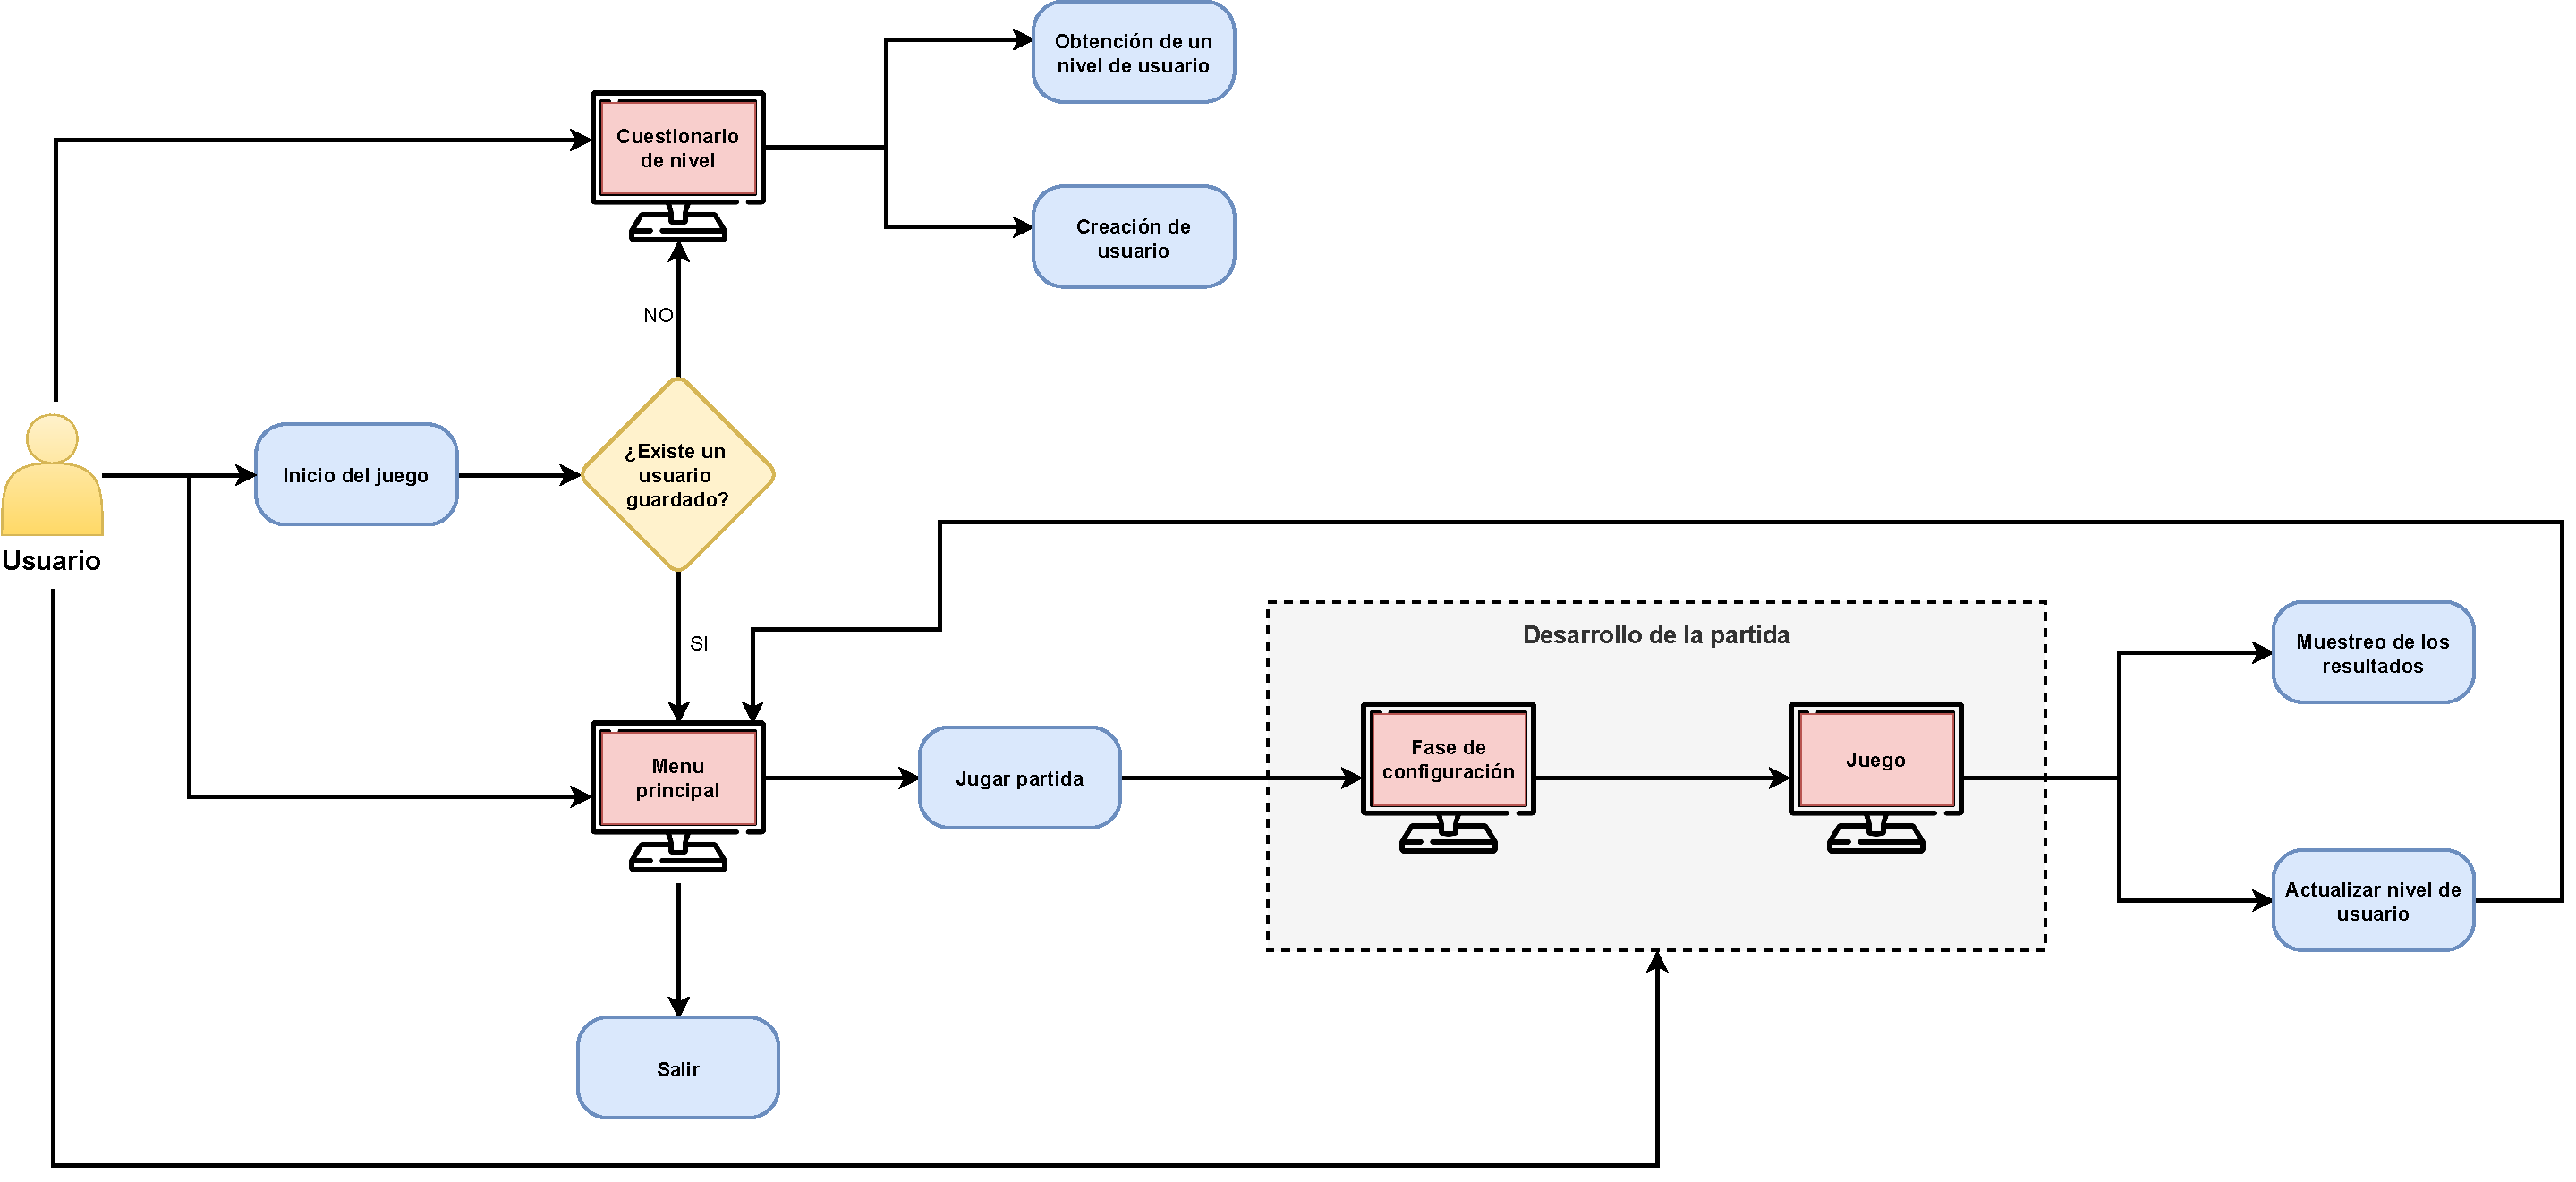
\includegraphics[width=0.95\linewidth]{FuncionamientoJuego}
	\caption[Funcionamiento de GLOBAL-MANAGER]{Diagrama del funcionamiento del JS propuesto, GLOBAL-MANAGER}
	\label{fig:funcionamientoJuego}
\end{figure}

Este TFG se enmarca dentro de un contrato I+D con el grupo de investigación Alarcos\footnote{\url{https://alarcos.esi.uclm.es}} de la Universidad de Castilla La-Mancha (UCLM)\footnote{\url{https://www.uclm.es/}}, en concreto en el proyecto "G3SOFT: Ingeniería de Modelos para el Gobierno y Gestión del Desarrollo Global de Software"\footnote{\url{https://alarcos.esi.uclm.es/proyectos/G3SOFT/index.php}}, el cual se centra en la mejora del gobierno y la gestión de proyectos de DGS. En la tab.~\ref{tab:ResumenG3SOFT} se muestra un resumen de dicho proyecto.

\begin{table}[htb]
	\centering
	\setlength{\arrayrulewidth}{0.5mm}
	\arrayrulecolor{white}
	\resizebox{\textwidth}{!}{
    \begin{tabular}{l | p{25.5em}}
        \rowcolor[rgb]{.082, .082, .565} \textcolor[rgb]{1, 1, 1}{\textbf{Nombre:}} & \cellcolor[rgb]{.753, .753, .753}G3SOFT:Ingeniería de Modelos para el Gobierno y Gestión del\newline{}Desarrollo Global de Software \\ \hline
        \rowcolor[rgb]{.082, .082, .565} \textcolor[rgb]{1, 1, 1}{\textbf{Financiación:}} & \cellcolor[rgb]{.753, .753, .753}JJCM Consejería de Educación y Cultura y Deportes, y Fondos\newline{}FEDER \\ \hline
        \rowcolor[rgb]{.082, .082, .565} \textcolor[rgb]{1, 1, 1}{\textbf{Referencia:}} & \multicolumn{1}{l}{\cellcolor[rgb]{.753, .753, .753}SBPLY/17/180501/000150} \\ \hline
        \rowcolor[rgb]{.082, .082, .565} \textcolor[rgb]{1, 1, 1}{\textbf{Dirección WEB:}} & \multicolumn{1}{l}{\cellcolor[rgb]{.753, .753, .753}\url{https://alarcos.esi.uclm.es/proyectos/G3SOFT/index.php}} \\ \hline
        \rowcolor[rgb]{.082, .082, .565} \textcolor[rgb]{1, 1, 1}{\textbf{Grupo de investigación:}} & \multicolumn{1}{l}{\cellcolor[rgb]{.753, .753, .753}Grupo Alarcos} \\ \hline
        \rowcolor[rgb]{.082, .082, .565} \textcolor[rgb]{1, 1, 1}{\textbf{Universidad colaboradora:}} & \multicolumn{1}{l}{\cellcolor[rgb]{.753, .753, .753}Universidad de Castilla-La Mancha (UCLM)} \\ \hline
    	\rowcolor[rgb]{.082, .082, .565} \textcolor[rgb]{1, 1, 1}{\textbf{Investigadores principales:}} & \cellcolor[rgb]{.753, .753, .753}Francisco Ruiz Gónzalez\newline{}Aurora Vizcaíno Barceló \\ \hline
    \end{tabular}}
	\caption{Características del proyecto G3SOFT}
	\label{tab:ResumenG3SOFT}
\end{table}


\section{Estructura del documento}
\label{sec:Estructura}

A continuación, se define la estructura del documento, la cual hace referencia a la memoria del TFG y esta dividida en los siguientes capítulos:

\begin{itemize}
	\item \textbf{Capítulo 1. Introducción:} breve resumen sobre la motivación, contexto y problemática que engloba este TFG, al igual que la solución que se propone.
	\item \textbf{Capítulo 2. Objetivos:} listado tanto del objetivo principal como los objetivos secundarios que se persiguen con la realización de dicho TFG, además de las tareas necesarias para llevarlo a cabo.
	\item \textbf{Capítulo 3. Estado del arte:} información referente sobre el DGS, la gestión y administración de proyectos DGS, de igual modo se especifican un conjunto de habilidades, las cuales son necesarias para llevar a cabo el trabajo de jefe de proyecto software en un entorno distribuido. Por último, se define e indica la importancia de la gamificación en general, y de los JS en particular, a su vez de una serie de ejemplos sobre JS relacionados con el tema de este TFG.
	\item \textbf{Capítulo 4. Método de trabajo:} especificación de la metodología de trabajo que se seguirá para el desarrollo de este TFG, al igual que las herramientas y tecnologías (tanto software como hardware) que se utilizarán en dicho periodo.
	\item \textbf{Capítulo 5. Resultados:} informe de los resultados obtenidos tras llevar a cabo cada uno de los objetivos y tareas definidas en el capítulo 2, utilizando el método de trabajo definido en el capítulo 4, al igual que todos los posibles problemas e impedimentos que puedan haber surgido en la realización de este TFG.
	\item \textbf{Capítulo 6. Conclusiones:} exposición de la conclusión y trabajos futuros tras haber realizado el presente TFG, del mismo modo que las lecciones aprendidas y una valoración personal.
	\item \textbf{Bibliografía:} sinopsis de las fuentes de información consultadas para la realización de este TFG.
\end{itemize}